\section{Maxwell’schen Gleichungen}

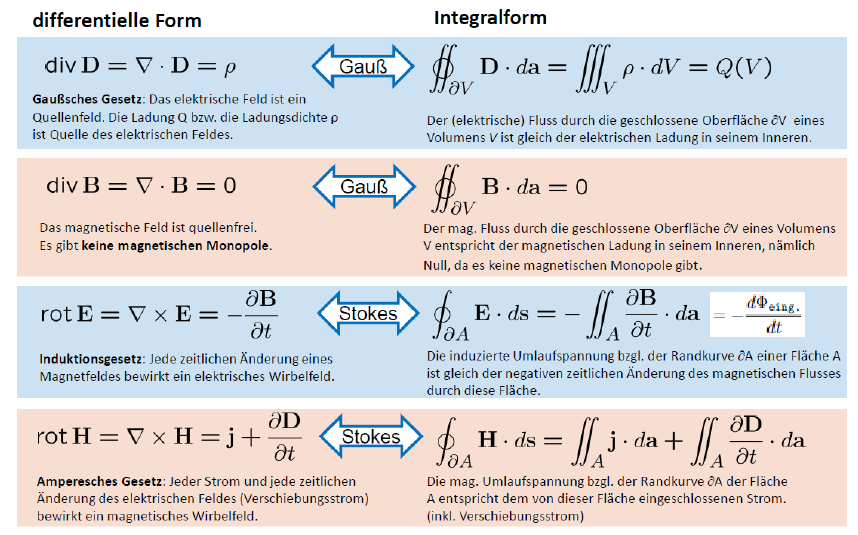
\includegraphics[width=\columnwidth]{Figures/Integralsatz.png}

\textbf{Aussage Durchflutungssatz:}

\begin{tabularx}{\textwidth}{>{\hsize=.5\hsize}X>{\hsize=.5\hsize}X}
    Elektrischer Strom ist Ursache für magnetische Wirbelfeld & $\boxed{\int_c \vec{H} d \vec{s} = I = \iint_A \vec{J} d \vec{A}}$ \\
    Bewegte elektrische Ladung erzeugt Magnetfeld       & $\boxed{ rot \vec{H} = \vec{J} = \sigma \cdot \vec{E}} $
\end{tabularx}

Bei isotropen Stoffen sind $\varepsilon$ u. $\mu$ Skalare:
\[
    \varepsilon = \varepsilon_0 \cdot \varepsilon_r \qquad \mu = \mu_0 \cdot \mu_r
\]

\subsection{Integralsätze}
\begin{description}
    \setlength{\itemsep}{1pt}
    \item Fundamentalsatz der Analysis
    \item Gauß: Vektorfeld das aus Oberfläche von Volumen strömt muss aus Quelle in Volumen
    \item Stokes: innere Wirbel kompensieren $\rightarrow$ Rand betrachten
\end{description}
\begin{align*}
    \int_{a}^b \opgrad F \cdot d \vec{s}     & = F(b) - F(a)                                  \\
    \iiint_V \opdiv \vec{A} \cdot dV         & = \oiint_{ \partial V} \vec{A} \cdot d \vec{a} \\
    \iint_{A} \oprot \vec{A} \cdot d \vec{a} & = \oint_{ \partial A} \vec{A} \cdot d \vec{r}
\end{align*}
